
\FloatBarrier\begin{figure}[!h]
\centering
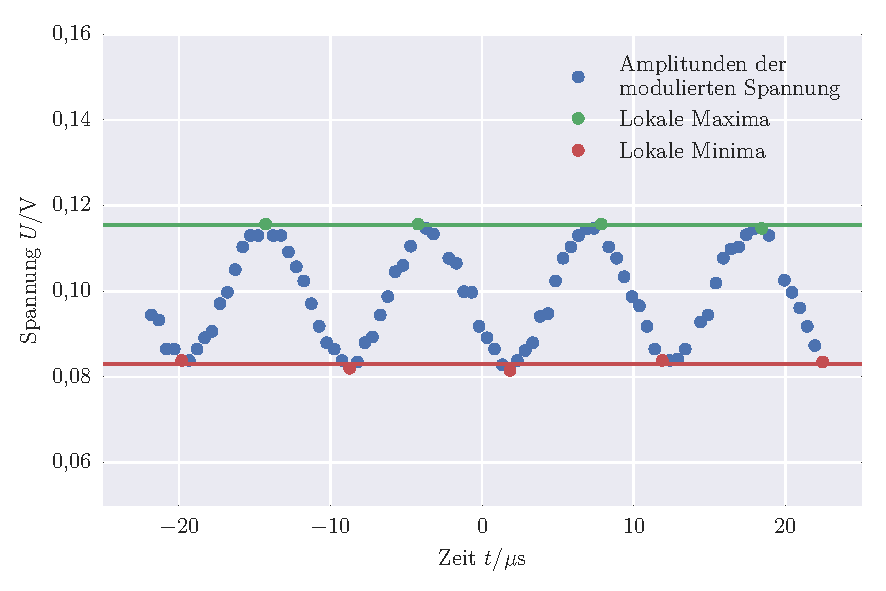
\includegraphics[scale=1]{../Grafiken/Amplituden_Modulierte_Spannung_mit_Traeger_Modulationsgrad.pdf}
\caption{Amplituden der amplitudenmodulierten Spannung aus \cref{fig:amplituden_modulierte_spannung_mit_traeger}.
Farblich hervorgehoben sind jeweils die lokalen Extrema. Die abgebildet Geraden markieren jeweils den Mittelwert
dieser Extremwerte.
 \label{fig:amplituden_modulierte_spannung_mit_traeger_modulationsgrad}}
\end{figure}
\FloatBarrier